\section{Deep Learning for Object Detection}
\label{sec:nn-objectdetection}
Object detection is fundamental computer vision problem visual recognition other
than as image classification, semantic segmentation. In particular object
detection not only recognize object categories but also predict the location of
each object by  bounding box. On the other hand semantic segmentation aims to
predict pixel-wise classifiers to assign a specific category label to each
pixel, thus providing an even richer understanding of an image. However, in
contrast to object detection, semantic segmentation does not distinguish between
multiple objects of the same category.\cite{wu2020recent}
Current state-of-the-art object detection systems are variants of the following
approach: hypothesize bounding boxes, re-sample pixels or features for each box,
and apply a high quality classifier.\\  
Although accurate, these approaches have
been too computationally intensive for embedded systems and, even with high-end
hardware, too slow for real-time or near real-time applications. Often detection
speed for these approaches is measured in seconds per frame, and even the
fastest high-accuracy detector, the basic Faster R-CNN, operates at only 7
frames per second (FPS). There have been a wide range of attempts to build
faster detectors by attacking each stage of the detection pipeline, but so far,
significantly increased speed comes only at the cost of significantly decreased
detection accuracy.\cite{liu2016ssd}
To derive a performance improvement translated into an increase in detection
speed with high precision ($58$ FPS with mAP $72.1\%$ on VOC2007 test, vs Faster
R-CNN $7$ FPS with mAP $73.2\%$ or YOLO $45$ FPS with mAP $63.4\%$). From this
derives the elimination of the proposals of delimitation boxes and of the
subsequent phase of re-filling of the pixels or of the characteristics.
Furthermore, the improvements introduced can be summarized in the use of a
convolution filter to predict the categories of objects and offsets in the
positions in the positioning of the panes, using separate predictors (filters)
for different aspect ratio detections, and applying these filters to multiple
features maps from the later stages of a network in order to perform detection
at multiple scales. \hfill \break
It is observed that With these modifications we can achieve
high-accuracy detection using relatively low resolution input, further
increasing processing speed. While these contributions may seem small
independently, we note that the resulting system improves accuracy on high-speed
detection for PASCAL VOC from $63.4\%$ mAP for YOLO to $72.1\%$ mAP for the
network used.\cite{liu2016ssd,Huang2016SpeedAccuracyTF}
So to ensure stability and portability of the model is used The API TensorFlow
Object Detection is an open source framework based on TensorFlow which
simplifies the construction, training and implementation of object detection
Templates.\cite{objectdetectionAPI}
%
%
\begin{figure}[!h]
	\centering
	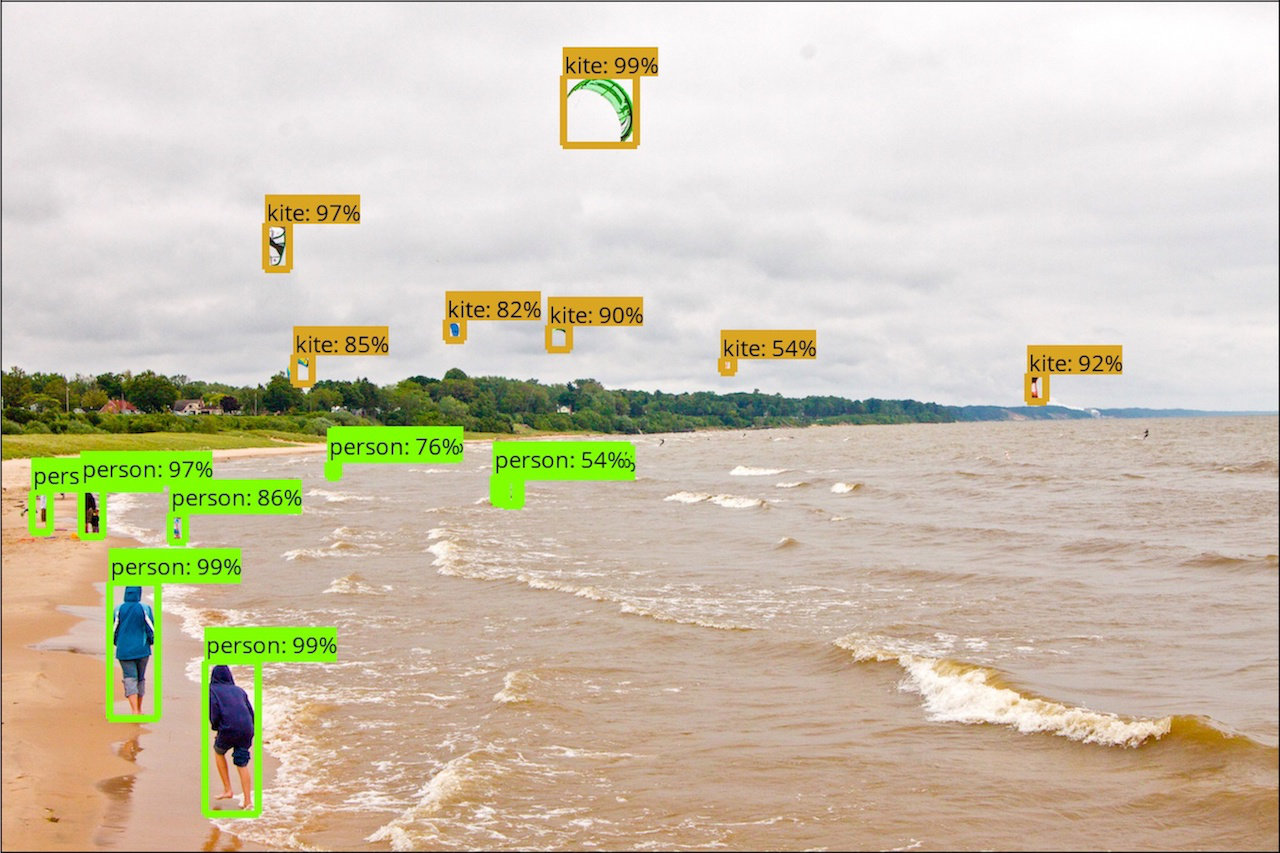
\includegraphics[width=0.75\textwidth]{kites_detections_output.jpg}
	\captionsource{example multiple object detection in a single image.}%
	{\href{https://github.com/tensorflow/models/tree/master/research/object_detection}{GitHub.com - TensorFlow}}
	\label{fig:kites-detections-output}
\end{figure}
%
%
\subsection{Single Shot Detector MobileNet}
\label{ssec:single-shot-detector}
The model of SSD in based on idea of we want detect the position of object
interest In addition to knowing what it is one who classified. To better
comprehension let's start from nomenclature:
\begin{description}
\item[Single Shot] The localization and classification operation must be single forward pass of the network.
\item[Multibox] Technique for bounding box regression.
\item[Detector] The neural network has the duty classifies those detected object.
\end{description}
%
The model \emph{SSD MobileNet} exploit four stages: the input layer for
importing the target image, the MobileNet base for extracting image features,
the SSD for classification regression and bounded box regression and the output
layer for exporting the detection result.\cite{Li_2018} 
The advantage of this net are speed and accuracy in detection task borrowed from
reduced compute complexity.
























% This section describes our proposed SSD framework for detection (Sec. 2.1) and the associated training methodology (Sec. 2.2). Afterwards, Sec. 3 presents dataset-specific model details and experimental results.

% 2.1 Model
% The SSD approach is based on a feed-forward convolutional network that produces a fixed-size collection of bounding boxes and scores for the presence of object class instances in those boxes, followed by a non-maximum suppression step to produce the final detections. The early network layers are based on a standard architecture used for high quality image classification (truncated before any classification layers), which we will call the base network1. We then add auxiliary structure to the network to produce detections with the following key features:
% Multi-scale feature maps for detection We add convolutional feature layers to the end of the truncated base network. These layers decrease in size progressively and allow predictions of detections at multiple scales. The convolutional model for predicting detections is different for each feature layer (cf Overfeat[4] and YOLO[5] that operate on a single scale feature map).
% Convolutional predictors for detection Each added feature layer (or optionally an ex- isting feature layer from the base network) can produce a fixed set of detection predic- tions using a set of convolutional filters. These are indicated on top of the SSD network architecture in Fig. 2. For a feature layer of size m × n with p channels, the basic element for predicting parameters of a potential detection is a 3 × 3 × p small kernel that produces either a score for a category, or a shape offset relative to the default box coordinates. At each of the m × n locations where the kernel is applied, it produces an output value. The bounding box offset output values are measured relative to a default box position relative to each feature map location (cf the architecture of YOLO[5] that uses an intermediate fully connected layer instead of a convolutional filter for this step).
% Default boxes and aspect ratios We associate a set of default bounding boxes with each feature map cell, for multiple feature maps at the top of the network. The default boxes tile the feature map in a convolutional manner, so that the position of each box instance relative to its corresponding cell is fixed. At each feature map cell, we predict the offsets relative to the default box shapes in the cell, as well as the per-class scores that indicate the presence of a class instance in each of those boxes. Specifically, for each box out of k at a given location, we compute c class scores and the 4 offsets relative to the original default box shape. This results in a total of (c + 4)k filters that are applied around each location in the feature map, yielding (c + 4)kmn outputs for a m × n feature map. For an illustration of default boxes, please refer to Fig. 1. Our default boxes are similar to the anchor boxes used in Faster R-CNN [2], however we apply them to several feature maps of different resolutions. Allowing different default box shapes in several feature maps lets us efficiently discretize the space of possible output box shapes.
